

\section{Programs}
Every example program in this section uses R7 as a stack pointer which is initialised to the by the program to 0x07D0.% using the LUI and LLI instructions.
The simulation environment contains an area of an area of memory with $2048$ locations and memory mapped deices.
There are $16$ switches at location $0$x$0800$, $16$ LEDs at location $0$x$0801$ and a serial io device which can be read from location $0$x$A000$ and has a control register at location $0$x$A001$. 




\subsection{Multiply}
\label{sec:multiply}
The code for the multiply program is held in Appendix~\ref{sec:multiply_appendix} listing~\ref{lst:multiply.asm}.
A sixteen bit number is read from input switches, split in to lower and upper bytes which are then multiplied.
The resulting sixteen bit word is written to the LEDs before reaching a terminating loop.
Equation~\eqref{eqn:multi} formally describes the algorithm disregarding limitations.

\begin{equation}
	A = M \times Q = \sum_{i=0}^{\infty} 2^i M_i Q\:\:where\:\:M_i \in \{0,1\}
   \label{eqn:multi}
\end{equation}



The subroutine operation is described in listing~\ref{lst:multiply.c}, using C. 
If the result is greater than or equal to $2^{16}$ the subroutine will fail and return zero.
The lowest bit of the multiplier controls the accumulator and the overflow check.
The multiplier is shifted right and the quotient is shifted left at every iteration.
An unconditional branch is used to keep the algorithm in a while loop. 
The state of the multiplier is compared at every iteration against zero when the algorithm is finished.
As size of the multiplier controls the number of iterations a comparison is made on entry to use the smallest operand.

\lstinputlisting[style=C,label=lst:multiply.c,caption=Multiply Subroutine]{pseudocode/multiply.c}



%The multiply code has also been optimised by unrolling the loop contents and is held in Appendix~\ref{sec:multiply_unrolled_appendix} listing~\ref{lst:multiplyUnroll.asm}.
%In implementation a trade off between code size and execution time is made by loop unrolling the eight stages.
%This creates scope for optimisation in operations contained in the loop, doesn't use a counter and requires less branch operations.





\subsection{Factorial}
\label{sec:factorial}
The code for the factorial program is held in Appendix~\ref{sec:factorial_appendix} listing~\ref{lst:factorial.asm}.
It is possible to calculate the factorial of any integer value between $0$ and $8$ inclusive.
The subroutine is called which in turn calls the multiply subroutine discussed in section~\ref{sec:multiply}. 
The factorial subroutine does no parameter checking but the multiply code does so if overflow does occur zero is propagated and returned; zero is not a possible factorial.
The result is calculated recursively as described using C in listing~\ref{lst:factorial.c}.
Large values can cause stack overflow the main body of code makes sure inputs, read from the switches, are sufficiently small.

\lstinputlisting[style=C,label=lst:factorial.c,caption=Recursive Factorial Subroutine]{pseudocode/factorial.c}






\subsection{Random}
The code for the random program is held in Appendix~\ref{sec:random_appendix} listing~\ref{lst:random.asm}.
A random series of numbers is achieved by simulating the $16$ bit linear feedback shift register in Figure~\ref{fig:lfsr}. 
This produces a new number every $16$ sixteen clock cycles so in this case a simulation subroutine is called $16$ times.
A seed taken from switches and passed to the first subroutine call via the stack is altered and passed to the next subroutine call.
No more stack operations are performed.
A load from the stack pointer is used write a new random number to LEDs.
All contained within an unconditional branch but a loop counter is used control write and reset.

\begin{figure}[ht]
   \centering
    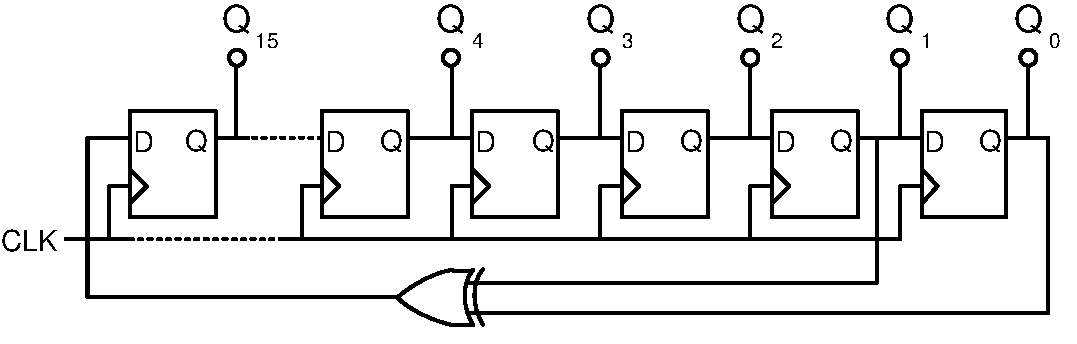
\includegraphics[width = 0.8\textwidth]{LFSR.pdf}
		\caption{16 Bit Linear Feedback Shift Register.}% \todo[inline]{Maybe change to IEEE symbols if we have time, AJR: we still have the eagle d-types but I think it would look a bit messy} }
   \label{fig:lfsr}
\end{figure}

A two input XOR gate is simulated using the XOR operation along with shifting to compare bits in different locations.
Bits $2$ and $4$ are used as inputs so a logical shift left by two is used to align them at the bit $4$ position. 
Masking the output value is used feedback to the top bit.
This is described using C in listing~\ref{lst:random.c}. 

\lstinputlisting[style=C,label=lst:random.c,caption=Linear Feedback Shift Register Subroutine]{pseudocode/random.c}





\subsection{Interrupt}
The code for the interrupt program is held in Appendix~\ref{sec:interrupt_appendix} listing~\ref{lst:interrupt.asm}.
This is the most complex example and makes use of both the multiply and factorial subroutines in sections~\ref{sec:multiply} and~\ref{sec:factorial} respectively.
The interrupt services the serial device by writing data to a $4$ byte circular buffer. 
A main program check to see if data is in the buffer then and if so calculates the factorial writing the result to the LEDs.
The buffer is purposefully small to test overflow.

\lstinputlisting[style=C,label=lst:interrupt.c,caption=Serial Device Interrupt Service Request]{pseudocode/interrupt.c}




